\documentclass[a4paper,12pt]{article}
\usepackage[T1]{fontenc}
\usepackage[utf8]{inputenc}
\usepackage{lmodern}
\usepackage[francais]{babel}

\usepackage{fullpage}
\usepackage{subcaption}
\usepackage{graphicx}
\usepackage{fancyhdr}
\usepackage{xcolor}
\usepackage{fancyhdr}
\usepackage{lastpage}
\usepackage{calc}
\setlength\voffset{-20pt}
\setlength\headheight{60pt}
\setlength\footskip{80pt}
\setlength\headsep{30pt}
\setlength\textheight{\textheight-100pt}

\def\companylogo{\rule{2cm}{2cm}}
\fancypagestyle{companypagestyle}{
    \fancyhf{}
    
    \fancyhead[C]{Implémentation du PageRank avec MPI \\}
    
    \fancyhead[R]{
      \parbox[b]{3cm}{
\includegraphics[width=3cm]{centrale.jpg}}}
    
    \fancyfoot[L]{
      \parbox[b]{\dimexpr\linewidth\relax}{
        Page \thepage\ sur \pageref{LastPage} \hfill \textsc{High Performance Computing}\\
        {\rule{\dimexpr\linewidth\relax}{0.4pt}}\\
        Ayaz \textsc{Badouraly}}
    }
}

\pagestyle{companypagestyle}
\renewcommand{\baselinestretch}{1.2}

\usepackage{setspace}
\usepackage[hidelinks]{hyperref}
\usepackage{marvosym}
\usepackage{amsmath}
\usepackage{dsfont}
\usepackage{soul}
\usepackage{listings}
\lstdefinestyle{customc}{
  belowcaptionskip=1\baselineskip,
  breaklines=true,
  frame=L,
  xleftmargin=\parindent,
  language=C,
  showstringspaces=false,
  basicstyle=\footnotesize\ttfamily,
  keywordstyle=\bfseries\color{green!40!black},
  commentstyle=\itshape\color{purple!40!black},
  identifierstyle=\color{blue},
  stringstyle=\color{orange},
}

\title{Rapport de Calculs Intensifs\\Implémentation du PageRank avec MPI}
\author{}
\date{}

\begin{document}

\maketitle

\thispagestyle{empty}

\textit{Auteur} : Ayaz \textsc{Badouraly}

\textit{Date} : 13 avril 2016

\vspace{2cm}

\begin{figure}[h]  
  \centering
  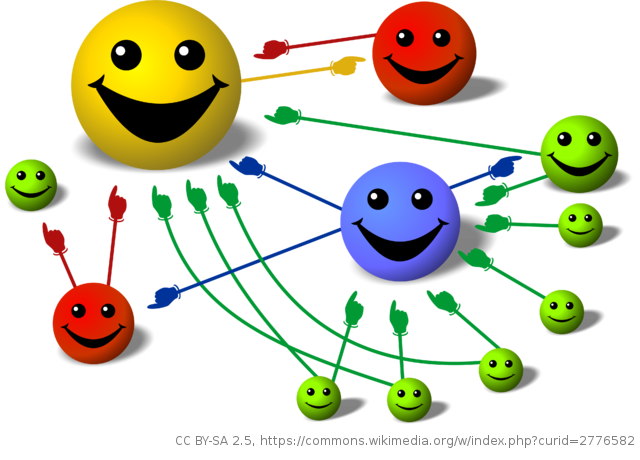
\includegraphics[width=.9\linewidth]{pagerank.png}
\end{figure}


\newpage

{\color{white}{.}}

\vspace{1cm}

\tableofcontents

\newpage

\section{Introduction}

Pour classer les pages web indépendamment de la sémantique, Sergey Brin et Lawrence Page ont conçu le \textit{pagerank} en 1998. 
L'idée était d'attribuer une note à une page, vue comme un sommet du graphe orienté du web. 
Le critère de classement sélectionné est alors purement quantitatif et repose sur les liens entre les différents n\oe{}uds.

\bigskip

Malgré la simplicité de l'idée sous-jacente au pagerank, la taille du graphe du web ne permet pas de calculer son pagerank en un temps raisonnable sur un seul c\oe{}ur d'une seule machine, aussi puissante soit-elle.

Je propose ici une implémentation parallèle et distribuée de l'algorithme du pagerank, utilisant la librairie \texttt{MPI} (~\textit{Message Passing Interface}~).

\bigskip

Ce rapport a pour but de présenter le travail que j'ai effectué entre le vendredi 4 mars et le mercredi 13 avril. Il s'agit d'un support au code source lui-même. Les points les plus subtiles du code source sont expliqués sous forme de commentaires directement dans les fichiers sources.

\newpage

\section{Algorithme du PageRank}

\subsection{Définition du \textit{pagerank}}

On considère un graphe orienté $G = (U, L)$ où $U$ est l'ensemble des sommets du graphe, et $L$ l'ensemble des arcs.  

\bigskip

Par analogie à la matrice d'adjacence de $G$, on définit la transposée de la matrice d'adjacence normalisée $A = (a_{ij})$ de $G$ telle que :
$$
\forall (i,j) \in U \times U : a_{ij} = \left\{
\begin{array}{ll}
  \frac{1}{\#(j)} & \text{si } (j,i) \in L \\
  0 & \text{sinon}
\end{array}
\right.
$$  
où $\#(j)$ est le nombre de liens sortants du sommet $j$.
$A$ représente \ul{le surfeur qui navigue de proche en proche en cliquant sur un lien au hasard de la page dans laquelle il se trouve}.

\bigskip

Pour modéliser \ul{le surfeur qui arrive sur une page puit (~\textit{ie.} sommet sans arc sortant~) et qui va sur une page quelconque ensuite}, on introduit la matrice $D = (d_{ij})$ telle que :
$$
\forall (i,j) \in U \times U : d_{ij} = \left\{
\begin{array}{ll}
  \frac{1}{\text{card}(U)} & \text{si } d^+(j) = 0 \\
  0 & \text{sinon}
\end{array}
\right.
$$
où $d^+(j)$ est le degré sortant du sommet $j$.

\bigskip

Enfin, pour modéliser \ul{le surfeur qui se lasse et qui va sur une nouvelle page au hasard}, on introduit la matrice $E = ( \frac{1}{\text{card}(U)} )$ de la même dimension que les matrices précédentes et qui ne contient que le terme $\frac{1}{\text{card}(U)}$.

\bigskip

La matrice de changement de distribution $M$ est alors définie comme :
$$ M = dA + dD + (1-d)E $$
où $d$ est le \textit{damping factor} ; $d$ vaut usuellement $0,85$.

\bigskip

Le vecteur pagerank $p$ est définit comme l'unique vecteur à valeurs positives, unitaire pour la norme $\Vert \cdot \Vert _1$ et vérifiant : 
\begin{equation}
  Mp = p
  \label{eq:pagerank}
\end{equation}

\subsection{Explication de l'algorithme}

Plutôt que de résoudre analytiquement l'équation (~\ref{eq:pagerank}~), nous allons approximer la solution.

\bigskip

On définit la suite récurrente :

$$
\left\{
\begin{array}{llcl}
   & p^0 & = & \begin{pmatrix}
     \frac{1}{\text{card}(U)} \\
     \vdots \\
     \frac{1}{\text{card}(U)}
   \end{pmatrix}\\
  \forall n \in \mathds{N} : & p^{n+1} & = & M p^n 
\end{array}
\right.
$$

On se donne un seuil de précision $\varepsilon$.

\bigskip

L'algorithme consiste à calculer petit à petit la suite $(p^0, p^1, p^2, \cdots )$, jusqu'à trouver $N \in \mathds{N}$ tel que :
$$ \left\Vert p^{N+1} - p^N \right\Vert < \varepsilon $$ 
$p^N$ est alors une bonne approximation du pagerank $p$.

\bigskip

Puisque nous sommes en dimension finie, les normes sont équivalentes.
J'ai donc choisi d'utiliser la norme infinie pour le calcul des distances, afin que la précision du calcul du pagerank soit directement liée à la précision de chacune de ses composantes.

\subsection{Justification mathématique}

Par construction, ${}^t M$ est une matrice stochastique. Donc 1 est valeur propre de ${}^t M$. De plus, ${}^t M$ est de norme subordonnée 1. On en déduit que le rayon spectral de ${}^t M$ vaut 1.

\bigskip

Les éléments de la matrice ${}^t A+{}^t D$ ne sont pas nécessairement tous strictement positifs, mais au moins positifs. Les éléments de la matrice ${}^t E$ sont tous strictements positifs. On en déduit que la matrice ${}^t M$ est primitive.

\bigskip

Le théorème de Perron-Frobenius permet de conclure sur l'existence et l'unicité du pagerank : c'est le vecteur de Perron-Frobenius.

\bigskip

Par ailleurs, cela montre que 1 est une valeur propre simple de ${}^t M$. La convergence de la suite $(p^n)$ vers $p$ est donc garantie, en tant que probabilité stationnaire de la chaîne de Markov de matrice de transition de ${}^t M$ irréductible.

\newpage

\section{Implémentation}

\lstset{style=customc}

Concernant l'arborescence du répertoire, les fichiers sont séparés enre le dossier \texttt{src/} pour les sources principales (~\texttt{src/main.c} et \texttt{src/pagerank.c}~), le dossier \texttt{lib/} pour les librairies (~\texttt{lib/file.c}, \texttt{lib/ma\-trix.c} et \texttt{lib/vector.c}~) et le dossier \texttt{tests/} pour les tests unitaires.

Les entrées du programme se trouvent dans le dossier \texttt{input/} et les sorties dans le dossier \texttt{output/}.

\bigskip

La compilation\footnote{\textit{N.B.:} travaillant sous Linux, je garantis le fonctionnement sur cet OS \textemdash $ $ et plus généralement sur tout OS certifié POSIX \textemdash $ $ mais pas sur Windows (~j'ai tout de même ajouté quelques instructions préprocesseurs concernant cet OS~). Si besoin, je suis en mesure de fournir une machine Linux fonctionnelle.} est automatisée grâce à un \texttt{Makefile}.
Les exécutables sont générés dans le dossier \texttt{bin/} avec l'extension \texttt{.run}.

\subsection{Structures de données}

Dans tout le projet, les quantités sont des nombres flottants à double précision. En C, ils sont implémentés avec le mot-clé : \texttt{double}.

\subsubsection{Représentation des vecteurs}

Les vecteurs sont représentés sous forme de tableaux unidimensionnels de \texttt{double}.

\bigskip

Le fichier \texttt{lib/vector.h} contient la définition de la structure \texttt{Vector}. Elle contient un entier pour le nombre de composantes et un tableau alloué dynamiquement.

\bigskip

\begin{lstlisting}
struct Vector
{
	int dim;
	double *vector;
};
\end{lstlisting}

\vspace{2cm}

\subsubsection{Représentation des matrices}

Les matrices considérées dans le problème du PageRank sont grandes et creuses\footnote{\textit{cf.} la visualisation des matrices sous forme d'images PNG.}. Les stocker sous forme de tableaux bidimensionnels est donc très coûteux en espace. J'ai donc fait une implémentation des matrices sous la forme COO (~\textit{coordinate format}~).

\bigskip

Le fichier \texttt{lib/matrix.h} contient la définition de la structure \texttt{COO$\_$Matrix}. Elle con\-tient un entier pour le nombre de composantes non nulles, deux tableaux de \texttt{int} alloués dynamiquement contenant les index \textit{i} et \textit{j} des composantes non nulles, et un tableau de \texttt{double} alloué dynamiquement contenant la valeur des composantes.

\bigskip

\begin{lstlisting}
struct COO_Matrix
{
	int nnz;
	int *rows;
	int *cols;
	double *values;
};
\end{lstlisting}

\medskip

Puisque c'est la seule forme de matrices utilisée dans le projet, j'ai mappé le mot-clé \texttt{Matrix} au mot \texttt{COO$\_$Matrix} :

\begin{lstlisting}
#define Matrix COO_Matrix
\end{lstlisting}

\medskip

\subsection{Les librairies ( \texttt{lib/} )}

\subsubsection{\texttt{lib/file.h}}

Ce fichier contient toutes les fonctions utiles pour intéragir avec la mémoire dure : lecture du disque et écriture sur le disque.

\subsubsection{\texttt{lib/matrix.h}}

Ce fichier contient la définition de la structure \texttt{COO$\_$Matrix} sour forme de trois tableaux unidimentionnels. Les tableaux sont alloués dynamiquement. J'ai donc écrit un constructeur et un destructeur.

\begin{lstlisting}
struct COO_Matrix construct_coo_matrix ( const int nnz ); 
	/* create a null matrix with COO format */
void destruct_coo_matrix ( struct COO_Matrix *mtx );
	/* free memory space */
\end{lstlisting}

\medskip

Il est aussi possible de charger une matrice à partir d'un fichier du dossier \texttt{input/}. Le fichier doit respecter certaines contraintes énumérées dans la section \ref{sec:input}.

\begin{lstlisting}
struct COO_Matrix from_graphfile_coo_matrix ( const char *filename, 
	int *nodes_number ); /* create a null matrix with COO format 
	from a graph written in a file */
\end{lstlisting}

\medskip

Pour accéder à un élément de la matrice, on passe par la fonction \texttt{get$\_$value$\_$coo$\_$ma\-trix}. Cette fonction prend en entrée les index \textit{i} et \textit{j}. S'il existe $k < \texttt{nzz}$ tel que $\texttt{rows}[k] = i$ et $\texttt{cols}[k] = j$, alors la fonction renvoie $\texttt{values}[k]$ ; sinon elle renvoie \texttt{0}.

\bigskip

J'ai écrit d'autres méthodes pour pouvoir intéragir plus facilement avec la structure de données (~ajout d'un élément à une matrice, sortie écran, enregistrement dans un fichier, création d'une copie~).

\bigskip

Dans le problème du PageRank, avoir une visualisation graphique de la matrice de transition d'une page à une autre. Ne serait-ce que pour \og voir \fg{} sur quoi l'on travaille. J'ai donc écrit une fonction créant une image en noir et blanc de la dimension de la matrice : chaque pixel noir représente une composante nulle de la matrice, et chaque pixel blanc représente une composante non nulle.
\begin{lstlisting}
#ifdef WITH_LIBPNG
int draw_coo_matrix ( const struct COO_Matrix *mtx, 
       const char *filename ); /* create a picture of a COO matrix */
#endif
\end{lstlisting}

Dans le \texttt{Makefile}, si la variable \texttt{WITH$\_$LIBPNG} vaut \texttt{yes}, l'édition de liens est exécutée avec l'option \texttt{-lpng}. Dans le code, on ajoute les headers :

\begin{lstlisting}
#ifdef WITH_LIBPNG
#include <png.h>
#endif
\end{lstlisting}
 La boucle principale est :
\begin{lstlisting}[numbers=left]
	for ( int i = 0 ; i < dim ; ++i ) {
		#pragma omp parallel for
		for ( int j = 0 ; j < dim ; ++j ) {
			if ( get_value_coo_matrix(mtx, i, j) ) {
				row[j] = 0xff;
			}
			else {
				row[j] = 0x00;
			}
		}
		png_write_row(png_ptr, row);
	}
\end{lstlisting}
Expliquons ce code : 
\begin{description}
  \item[variables en jeu]$ $
  \begin{description}
    \item[\texttt{mtx}]la matrice dont on trace une visualisation
    \item[\texttt{dim}]dimension de la matrice
    \item[\texttt{row}]une ligne de l'image, tableau de pixels de dimension \texttt{dim}
    \item[\texttt{png$\_$ptr}]pointeur vers l'image PNG que l'on est en train de construire
  \end{description}
  \item[lignes 4, 5 et 6]$ $\\si la matrice a une composante de coordonnées (\textit{i}, \textit{j}) non nulle, on ajoute un pixel blanc à la ligne \texttt{row}
  \item[lignes 7, 8 et 9]$ $\\sinon, on ajoute un pixel noir à la ligne \texttt{row}
  \item[ligne 11]$ $\\on écrit la ligne \texttt{row} dans l'image ; les appels à \texttt{png$\_$write$\_$row} doivent se faire dans le sens des \textit{i} croissant, donc les boucles ne sont pas interchangeables et encore moins parallélisables
  \item[ligne 2]$ $\\il n'y a aucune dépendance de données ou de sortie, donc la boucle de la ligne 3 à 11 est parallélisable ; pour cette petite boucle, j'ai voulu essayer \texttt{OpenMP} : dans le \texttt{Makefile}, on ajoute l'option \texttt{-fopenmp} au compilateur et à l'éditeur de liens
\end{description}


\subsubsection{\texttt{lib/vector.h}}

Il s'agit d'un librairie analogue à \texttt{matrix.h}. Même si les structures diffèrent, les méthodes sont quasiment identiques.

\bigskip

Ce fichier contient la définition de la structure \texttt{Vector} sour forme de tableau unidimentionnel. Le tableau est alloué dynamiquement. J'ai donc écrit un constructeur et un destructeur pour faciliter l'utilisation de la structure.

\begin{lstlisting}
struct Vector construct_vector ( const int dim );
	/* create a null matrix */
void destruct_vector ( struct Vector *vec );
	/* free memory space */
\end{lstlisting}

\medskip

Comme pour la structure \texttt{COO$\_$Matrix}, j'ai écrit des méthodes pour pouvoir intéragir plus facilement avec la structure de données (~accès à une composante, sortie écran, enregistrement dans un fichier, création d'une copie~).

Pour l'algorithme du PageRank, nous avons aussi besoin de calculer la distance entre deux vecteurs :

\begin{lstlisting}
double distance_vector ( const struct Vector *vec1, 
			 const struct Vector *vec2 );
\end{lstlisting}

\medskip

\subsection{Les sources ( \texttt{src/} )}

Chacune des sources, contenue dans le dossier \texttt{src/}, utilise les librairies définies plus haut. Lorsqu'elles sont compilées, le \texttt{Makefile} crée un exécutable \texttt{pagerank.run} dans le dossier \texttt{bin/}.

\bigskip

J'ai choisi d'adopter une structure de communication maître/esclaves. À l'initiation de la session \texttt{MPI}, un processus \texttt{root} est défini et il agira en tant que maître. Il ne fait aucun calcul sur les données, il envoie seulement des paramètres et des ordres aux autres processus qui sont de fait esclaves.

\subsubsection{\texttt{src/main.c}}

Le fichier \texttt{src/main.c} met en place les différents paramètres de calcul.

\bigskip

Dans la boucle \texttt{main}, la session \texttt{MPI} est initialisée (~\textit{cf. lignes 30 à 50}~) et le processus maître\footnote{Il est sauvegardé en mémoire dans la variable globale \texttt{root} \textemdash $ $ cette forme de variable est la plus simple à utiliser, car elle est utilisée dans plusieurs fichiers du projet et la passer en argument des fonctions l'utilisant s'avère être lourd en termes d'écriture.} est défini comme celui de plus grand numéro (~\textit{cf. ligne 40}~).

\bigskip

Ensuite, les options envoyées sont parsées (~\textit{cf. lignes 51 à 119}~).

\begin{description}
  \item[\texttt{-b <buffer$\_$size>}]$ $\\Prend en argument la taille du buffer\footnote{Elle est sauvegardée en mémoire dans la variable globale \texttt{buffer$\_$size}} ; c'est notamment utile lorsque le nom des sommets du graphe sont longs et que le parsing des fichiers \texttt{input/} échoue ;\\Si non utilisée, la valeur \texttt{BUFSIZ} est choisie
  \item[\texttt{-i <input$\_$filename>}]$ $\\Prend en argument un nom de fichier, dont on calculera le pagerank du graphe ;\\Si non utilisée, le nom du fichier est demandé interactivement (~\textit{cf. lignes 86 à 106}~)
  \item[\texttt{-p <precision>}]$ $\\Prend en argument la précision du pagerank souhaitée;\\Si non utilisée, la valeur par défaut est $10^{-6}$
  \item[\texttt{-h}]affiche l'aide
  \item[\texttt{-v}]active le mode \textit{verbose}\footnote{L'état \textit{verbose} est sauvegardé en mémoire dans la variable booléenne globale \texttt{verbose}}
\end{description}

Chaque processus aura besoin de connaître le nom du fichier d'entrée, on utilise donc un \texttt{MPI$\_$Bcast} pour transmettre la variable \texttt{input$\_$filename} (~\textit{cf. ligne 108}~).

\bigskip

Après avoir écrit sur le disque dur tous les paramètres (~\textit{cf. lignes 120 à 139}~), le calcul du pagerank est lancé (~\textit{cf. ligne 144}~) :

\begin{lstlisting}
compute_pagerank ( get_file_path(input_filename, INPUT), precision );
\end{lstlisting}

\medskip

L'utilisateur reçoit, en fonction du résultat, un message de réussite ou un message d'échec (~\textit{cf. lignes 144 à 153}~).

\vspace{2cm}

\subsubsection{\texttt{src/pagerank.c}}

Le fichier \texttt{src/pagerank.c} exécute le calcul effectif du pagerank. Grâce à l'ensemble des librairies, le code est court et explicite.

\bigskip

La première fonction appelée est \texttt{compute$\_$pagerank}. C'est la fonction principale. Elle renvoie \texttt{EXIT$\_$\-SUCCESS} si l'algorithme a convergé, \texttt{4} sinon.

\bigskip

Elle appelle \texttt{load$\_$graph} qui charge en mémoire la matrice COO transposée de la matrice d'adjacence du graphe du fichier \texttt{input$\_$filename}. 
La matrice est rendue stochastique en colonnes grâce à l'appel à la fonction \texttt{normalize}.

Dans un premier temps, la matrice est chargée seulement dans le processus \texttt{root}.

\bigskip

La matrice est ensuite partagée entre tous les processus grâce à la fonction \texttt{distri\-bute$\_$matrix}. 

Le processus \texttt{root} calcule dans un premier temps la taille des données à traiter par chaque processus\footnote{Le calcul est fait de manière intelligente, pour distribuer le plus également possible des données. Par exemple, s'il y a 10 données à distribuer sur 4 processus esclaves, alors les tailles calculées seront : $3 - 3 - 2 - 2$.} (~\textit{cf. lignes 131 à 140}~).

Le processus \texttt{root} fait quatre appels \texttt{MPI$\_$Send}, tandis que le processus esclave fait quatre appels \texttt{MPI$\_$Recv}. Les données tranférées sont : le scalaire \texttt{nnz} avec le tag $0$, le tableau \texttt{rows} avec le tag $1$, le tableau \texttt{cols} avec le tag $2$ et le tableau \texttt{values} avec le tag $3$.

\bigskip

Un pré-calcul est fait pour tenir compte du \textit{damping factor} avec la fonction \texttt{set$\_$damp\-ing$\_$factor}.

\bigskip

Une fois les données chargées en mémoire, le pagerank est calculé itérativement dans la fonction \texttt{launch$\_$computing}.
La boucle principale va de la ligne 258 à la ligne 286.

À chaque itération, tous les processus connaissent la valeur temporaire du pagerank dans la variable \texttt{pagerank}.

Chaque processus calcule le produit du pagerank par la matrice d'adjacence et le \textit{damping factor} avec la fonction \texttt{multiply$\_$matrix$\_$vector} (~\textit{cf. ligne 260}~). 
Chaque processus a donc en mémoire un vecteur dense \texttt{sub$\_$pagerank}, de dimension la taille du graphe, avec des composantes non nulles aux seules lignes dont le processus à la matrice. Le vecteur entier est donc reconstituable par un \texttt{MPI$\_$Allreduce} avec l'opérateur \texttt{MPI$\_$SUM} (~\textit{cf. ligne 263}~).

Le terme complémentaire du \textit{damping factor} est ajouté à la ligne 264.

À ce stade, tous les processus connaissent la valeur du pagerank à l'itération suivante dans la variable \texttt{next$\_$pagerank}.

Le processus \texttt{root} calcule la distance entre \texttt{pagerank} et \texttt{next$\_$pagerank}, et la communique à tous les processus (~\textit{cf. lignes 266 à 276}~).

Si la distance entre les deux vecteurs est inférieure à la précision souhaitée, le calcul s'arrête (~\textit{cf. lignes 278 à 281}~). 
Sinon, \texttt{pagerank} prend la valeur de \texttt{next$\_$pagerank} et le calcul est réitéré (~\textit{cf. ligne 283 à 285}~).
 
\subsection{Les data ( \texttt{input/} et \texttt{output/} )}

\subsubsection{\texttt{input/}}
\label{sec:input}

Le dossier \texttt{input/} contient toutes les données écrites en dur sur le disque et qui servent d'entrée aux différents programmes (~\textit{cf.} la librairie \texttt{lib/file.h}~).

\bigskip

Il s'agit de toutes les matrices, enregistrées en respectant les contraintes suivantes :  
\medskip
\begin{itemize}
  \item le fichier représente un graphe orienté, la matrice chargée en est la transposée du graphe d'adjacence
  \item les lignes commentées commencent par un \texttt{\#}
  \item la première ligne contient un entier représentant le nombre de sommets du graphe
  \item chaque autre ligne représente un arc entre deux sommets et est de la forme : \\ \texttt{node$\_$name$\_$1\textvisiblespace node$\_$name$\_$2}
  \item le graphe ne doit pas présenter de puit
\end{itemize}

\subsubsection{\texttt{output/}}
\label{sec:output}

Le dossier \texttt{output/} contient toutes les données écrites en dur sur le disque en sortie des programmes (~\textit{cf.} la librairie \texttt{lib/file.h}~).

\bigskip

Le dossier \texttt{output/} contient au moins trois fichiers :
\medskip
\begin{itemize}
  \item \texttt{settings.txt} qui contient les paramètres d'exécutions (~le fichier d'entrée, la précision du calcul et l'état de sortie du programme~)
  \item \texttt{mapping.txt} qui contient la correspondance entre les coordonnées du vecteur pagerank et le nom des n\oe{}uds (~\textit{cf.} les fichiers du dossier \texttt{input/}~)
  \item \texttt{pagerank.txt} qui contient le vecteur pagerank calculé, dans l'ordre croissant des coordonnées
\end{itemize}

\bigskip

Si demandé, le dossier \texttt{output/} contient aussi une image au format PNG représentant la matrice d'entrée.

\subsection{Les tests ( \texttt{tests/} )}

Le dossier \texttt{tests/} contient trois fichiers :
\medskip
\begin{itemize}
  \item \texttt{t$\_$pagerank.c} qui contient tous les tests unitaires des sources \texttt{src/pagerank.h}
  \item \texttt{t$\_$matrix.c} qui contient tous les tests unitaires de la librairie \texttt{lib/matrix.h}
  \item \texttt{t$\_$vector.c} qui contient tous les tests unitaires de la librairie \texttt{lib/vector.h}
\end{itemize}

\subsection{Codes d'erreur}

J'ai suivi une convention commune à tous les fichiers de \texttt{src/} et \texttt{lib/}. Si l'exécution se passe bien, une fonction va retourner \texttt{EXIT$\_$SUCCESS}, c'est-à-dire \texttt{0} sur la majorité des OS. Sinon :

\begin{description}
  \item[code d'erreur 1]$ $\\une erreur a été détectée sur les paramètres envoyés au programme
  \item[code d'erreur 2]$ $\\une erreur a été détectée lors d'un traitement sur un fichier ( ouverture, lecture, etc... ) 
  \item[code d'erreur 3]$ $\\le programme n'a pas été lancé avec un nombre cohérent de processus (~soit moins de deux, soit plus que la dimension du problème~)
  \item[code d'erreur 4]$ $\\l'algorithme du pagerank n'a pas convergé à la précision souhaitée après \texttt{MAX$\_$ITE\-RATION} itérations
\end{description}

Dans tous les cas, l'erreur est accompagnée d'un message explicatif pour faciliter le débuggage.

\bigskip

Une erreur provoque l'arrêt immédiat du processus par un \texttt{MPI$\_$Abort} ou par un \texttt{exit} non nul, ce qui provoque en conséquence l'arrêt de tous les processus lancés par \texttt{mpirun}.

\newpage

\section{Résultats}

\subsection{Exemple de pagerank : \texttt{interstices\_5}}

On travaille sur le graphe suivant :

\begin{figure}[h] 
  \centering 
  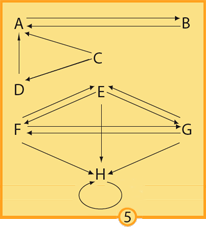
\includegraphics[scale=0.5]{interstices_5_graphe.png}
  \caption{Graphe interstices$\_$5}
\end{figure}

\bigskip

On obtient le mapping : 

\begin{itemize}
  \item index 0 (~coordonnée 1~) $\longmapsto$ n\oe{}ud A
  \item index 1 (~coordonnée 2~) $\longmapsto$ n\oe{}ud B
  \item index 2 (~coordonnée 3~) $\longmapsto$ n\oe{}ud C 
  \item index 3 (~coordonnée 4~) $\longmapsto$ n\oe{}ud D 
  \item index 4 (~coordonnée 5~) $\longmapsto$ n\oe{}ud E 
  \item index 5 (~coordonnée 6~) $\longmapsto$ n\oe{}ud F 
  \item index 6 (~coordonnée 7~) $\longmapsto$ n\oe{}ud G 
  \item index 7 (~coordonnée 8~) $\longmapsto$ n\oe{}ud H 
\end{itemize}
On constate qu'il respecte l'ordre alphabétique. Il s'agit d'un hasard lié à l'ordre des arcs du fichier \texttt{input/interstices$\_$5.txt}.

\bigskip

Avec un \textit{damping factor} de $0,85$, on obtient le pagerank en 72 itérations :

$$
  \begin{pmatrix}
    0,235557432433 \\
    0,218973817567 \\
    0,026718750000 \\
    0,018750000000 \\
    0,043269230769 \\
    0,043269230769 \\
    0,043269230769 \\
    0,370192307692
  \end{pmatrix}
$$
Le calcul théorique donne exactement ce pagerank avec une précision de $0,000000000001$.

\bigskip

\subsection{Exemple de matrice creuse : \texttt{p2p-Gnutella04}}

Voici un exemple de visualisation\footnote{Un pixel noir représente un élément nul, et un prixel blanc représente un élément non nul.} de matrice creuse, représentant un graphe de 10876 n\oe{}uds et 39994 arcs. L'image totale (~\ref{fig:matrice}~) contient si peu de points blancs qu'ils sont invisibles après redimensionnement de l'image. On les distingue sur l'extrait (~\ref{fig:sousmatrice}~) de celle-ci.

\bigskip

\begin{figure}[h] 
  \centering 
  \begin{subfigure}[c]{\linewidth}
    \centering
    \includegraphics[width=0.4\linewidth]{p2p-Gnutella04.png}
    \caption{Matrice totale $10876 \times 10876$}
    \label{fig:matrice}
  \end{subfigure} \\ \bigskip
\end{figure}
\begin{figure}
  \ContinuedFloat
  \begin{subfigure}[c]{\linewidth}
    \centering
    \includegraphics[width=0.9\linewidth, viewport= 0 10376 500 10876, clip=true]{p2p-Gnutella04.png}
    \caption{Extrait $500 \times 500$ de la matrice}
    \label{fig:sousmatrice}
  \end{subfigure}
  \bigskip
  \caption{Matrice d'adjacence du graphe p2p-Gnutella04}
\end{figure}

\newpage

\section{Conclusion}

\subsection{Synthèse du travail accompli}

Le code présenté dans le dossier est segmenté de sorte que ses différentes composantes indépendantes les unes des autres. Comme les librairies open-sources, elles pourront ainsi être réutilisées dans d'autres projets.

\bigskip

Il permet de répondre au cahier des charges en calculant le pagerank d'un graphe orienté, en utilisant la librairie \texttt{MPI}.

\subsection{Difficultés rencontrées}

Le langage C n'incluant pas la notion de surcharge de fonctions, il m'a été difficile de garder des notations claires, sans faire du code verbeux.

J'ai notamment essayé de cloisonner les librairies, en construisant des pseudo-objets à l'aide de structures et en fournissant de nombreuses fonctions s'apparentant aux méthodes du C++.

\bigskip

La partie sur la construction d'une image au format PNG a été la plus compliquée à mettre en place, à cause de l'absence de documentation claire. Néanmoins, je tenais à utiliser ce format d'images, notamment en raison des optimisations faites par les développeurs de la \texttt{libpng} qui permettent de stocker de grandes images sur peu d'espace mémoire.

\subsection{Pour aller plus loin}

Le travail présenté ici est un travail fait sur une petite échelle de temps. Il y a donc encore de nombreuses optimisations envisageables.

\bigskip

Du format de matrices COO que j'ai implémenté, on peut passer à un format CSR (~\textit{Compressed Sparse Row}~), car le tableau \texttt{rows} est ordonné.

Il est alors aisé d'effectuer les calculs non plus sur CPU, mais sur GPU, grâce à la librairie \texttt{cuSPARSE} de la \texttt{CUDA Toolkit}. Elle fournit des kernels déjà optimisés pour la multiplication d'une matrice creuse par une vecteur dense : \texttt{cusparseDcsrmv()}. Mon implémentation a l'avantage majeur de pouvoir appeler directement la fonction \texttt{cusparseDcoo2csr()} pour calculer la matrice CSR à partir de la matrice COO.

\bigskip

Sans aller jusqu'à la programmation sur GPU, il est possible d'améliorer l'algorithme de répartition de la matrice sur les différents processus, pour prendre en compte que certaines lignes contiennent plus d'éléments que d'autres. Ainsi, on gagnerait en homogénéité des temps d'occupation de chaque processus.

\bigskip

Il est également possible d'améliorer sensiblement la fonction \texttt{draw$\_$coo$\_$matrix} pour prendre en compte la structure de matrice au format COO. Mais cela implique de perdre le caractère parallélisable des boucles.

\bigskip

Pour mesurer la performance du programme, il serait intéressant de calculer et afficher le temps de calcul du programme. Il est même envisageable d'afficher le temps de calcul de chaque étape du code (~chargement des entrées, temps de chaque itération, etc...~)

\bigskip

Enfin, il est possible de tendre vers l'algorithme utilisé en production chez Google, en calculant un pagerank logarithmique sur une échelle de 0 à 10, plutôt qu'un pagerank linéaire sur une échelle de 0 à 1.

\newpage

\section{Bibliographie}

\bigskip

\begin{itemize}
  \item[{[1]}] \textit{The Anatomy of a Large-Scale Hypertextual Web Search Engine}, Sergey Brin and Lawrence Page, 1998, \url{infolab.stanford.edu/~backrub/google.html}
  \bigskip
  \item[{[2]}] \textit{Using your laptop to compute PageRank for millions of webpages}, Michael Nielsen, 2008, \url{michaelnielsen.org/blog/using-your-laptop-to-compute-pagerank-}\\\url{for-millions-of-webpages/}
  \bigskip
  \item[{[3]}] \textit{Le theorème de Perron-Frobenius, les chaines de Markov et un célèbre moteur de recherche}, Bachir Bekka, 2007, \url{agreg-maths.univ-rennes1.fr/documentation/docs/Perron-Frobenius.pdf}
  \bigskip
  \item[{[4]}] \textit{La formule de PageRank sur des exemples}, \\\url{interstices.info/encart.jsp?id=c_21839&encart=0&size=780,580}
  \bigskip
  \item[{[5]}] \textit{A description on how to use and modify libpng}, Glenn Randers-Pehrson, 2016, \url{www.libpng.org/pub/png/libpng-manual.txt}
  \bigskip
  \item[{[6]}] \textit{CUDA Toolkit Documentation}, \url{docs.nvidia.com/cuda/cusparse/}
\end{itemize}

\end{document}
